%!TEX root = main.tex

\section{Evaluation}
\label{sec:evaluation}
In the previous section, we describe the deployment scenarios we use to evaluate the broadcast algorithms.
%
In this section, we present the results of our experiments.
%
Such results are expressed in terms of the following metrics:

%
\noindent $\triangleright$
\textbf{Saved Rebroadcasts (SRE)} --
number of retransmissions we avoid by using an algorithm $A$ instead of \textit{simple flooding}\deleted{, which is considered the worst case}.
%
\deleted{To compute the SRE of one algorithm $A$ in a network of $N$ nodes, we measure the number $R_m$ of retransmissions made by $A$ to disseminate a message $m$. The $ \textit{SRE}_m$ for message $m$ is then $N - R_m$.}
%
\deleted{Since in our experiments we are disseminating many messages, we compute the mean \textit{SRE} and use it as metric for our comparison study.}
%
\deleted{This metric is useful to assess the performance of algorithms in terms of both network and energy usage. }

\noindent $\triangleright$
\textbf{Duplicate messages} --
number of times one broadcast message is received after its first reception.
%

\noindent $\triangleright$
\textbf{Reachability} --
percentage of nodes that successfully receive one broadcast message at least once.

\deleted{
\noindent $\triangleright$
\textbf{Broadcast time} --
time to disseminate one message with a reachability of 100\%.
}

% 
\noindent $\triangleright$
\textbf{Energy consumption} --
energy consumed by nodes during all broadcast session.
%
\begin{figure*}[ht]
	\begin{center}
	\subfigure[SRE messages in static scenarios.]{
		\label{fig:a-saved}
		
\includegraphics[page=1, scale=0.34, trim = 20mm 7mm 0 0]{fig/results-static-summary.pdf}
	}
	~
	\subfigure[Duplicate messages per algorithm in static scenarios.]{
		\label{fig:a-duplicated}
		
\includegraphics[page=3, scale=0.34, trim = 16mm 0 10mm 0]{fig/results-static.pdf}
	}
	~
	\subfigure[SRE messages in dynamic scenarios.]{
		\label{fig:b-saved}
		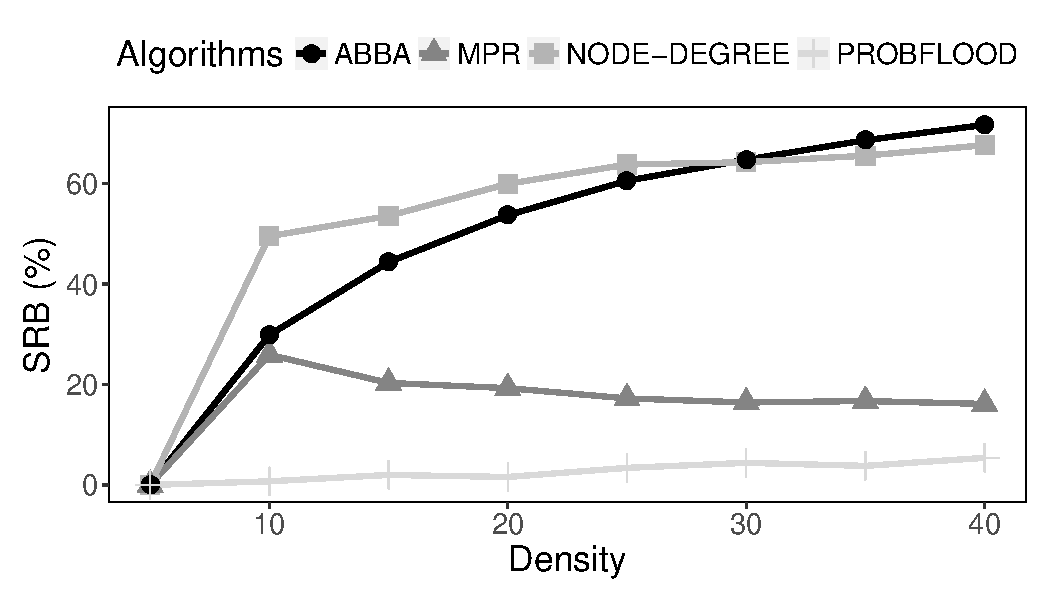
\includegraphics[page=1, scale=0.34, trim = 20mm 7mm 0 0]{fig/results-mobility-summary.pdf}
	}
	~
	\subfigure[Duplicate messages per algorithm in dynamic scenarios.]{
		\label{fig:b-duplicated}
		\includegraphics[page=3, scale=0.34, trim = 16mm 0 10mm 0]{fig/results-mobility.pdf}
	}
	\caption{Overload of wireless communication through \textit{SRE} and \textit{duplicate} messages.}
	\label{fig:saved-rebroadcasts}
	\end{center}
\end{figure*}


%
We study every metric with and without mobility over different densities as described in Section~\ref{sec:scenarios}.
%
\subsection{Network saturation}

The proportion of SRE and duplicate messages determine to which extent the communication medium is saturated.
%
Figure~\ref{fig:a-saved} depicts the SRE in static scenarios.
%
As can be seen, \textit{MPR} outperforms all other protocols.
%
However, the difference between \textit{MPR} and other algorithms decreases as the density increases.
%
Interestingly, \textit{ABBA} reduces the number of retransmissions more efficiently than the \textit{CDS-based} technique for densities above 10 but it does not surpass \textit{MPR}. 
%
The competitiveness of \textit{ABBA} was expected to increase with the density because \textit{ABBA} can then cancel more retransmissions, but it is surprising to see it outperforming \textit{CDS-based} by 10\%.
%

In dynamic scenarios, shown in Figure~\ref{fig:b-saved}, we observe that mobility affects the performance of topology-based algorithms -- particularly \textit{MPR}.
%
Indeed, nodes in \textit{MPR} and \textit{CDS-based} collects information about their neighbors that quickly becomes out of date due to the constant changes.
%
\deleted{Additionally, collisions of control messages in these algorithms is another explanation for the poor performance.}
%
Although \textit{ABBA} maintains its robustness when nodes moves, it requires a GPS whose power consumption is not considered in this paper.
%

The proportion of duplicate messages per algorithm is depicted in Figures~\ref{fig:a-duplicated} and~\ref{fig:b-duplicated}.
%
As this value varies per each broadcast session, we present a distribution of the metric.
%
In general, the lower the number of duplicate messages the better a protocol is in using the communication medium. 
%
However, in analyzing this metric, it is important to compare it against SRE because the occurrence of collisions also affects the received duplicate messages.
%
For instance, in the \textit{simple flooding} scenario with density 30, each node receives at most 10 duplicate messages instead of the expected 30.

%
\deleted{In general, there are three reasons to get a low number of duplicate messages: i) a higher value of SRE; ii) the occurrence of collisions; and iii) broadcast messages reach few peers (low reachability).}


%
The results on duplicate messages confirm that \textit{MPR} reduces network saturation in all scenarios.
%
Meanwhile, \textit{CDS-based} behaves similarly to \textit{ProbFlood} for low densities; but it outperforms \textit{ProbFlood} for density 20 and beyond.
%
\deleted{\textit{ProbFlood}'s behavior is specially poor in this metric, it is as bad as \textit{simple flooding} when the density is high.  }

\subsection{Power Consumption}

\deleted{Power consumption depends on the number of messages exchanged.}
%
The amount of received and sent messages is important for power consumption because every time a node exchanges messages \deleted{, the \textit{transmitter} and/or \textit{receiver} components of} its radio changes to a more power hungry mode.
%
Thus, both broadcast and control messages influence the energy consumption.
%
However, the network saturation in the vicinity of the node also influences the energy consumption due to the way the MAC layer is implemented.
%
In CSMA, a node keeps resending a message until the destination replies with an \textit{ACK} notification.
%
Although this strategy increases network reliability, it increments the energy consumption when the network is saturated.
%
Since in such a case packets are often lost, CSMA keeps resending messages and consuming energy in the process.
%

\begin{figure*}[ht]
	\begin{center}
	\subfigure[Reachebility in static scenarios]{
		\label{fig:a-coverage}
		
\includegraphics[page=2, scale=0.32, trim = 20mm 5mm 0 0]{fig/results-static-summary.pdf}
	}
	\hspace{0.2cm}
	\subfigure[Power consumption in static scenarios]{
		\label{fig:a-energy}
		
\includegraphics[page=1, scale=0.34, trim = 16mm 0 10mm 0]{fig/results-static.pdf}
	}
	~
	\subfigure[Reachebility in dynamic scenarios]{
		\label{fig:b-coverage}
		\includegraphics[page=2, scale=0.32, trim = 20mm 5mm 0 0]{fig/results-mobility-summary.pdf}
	}
	\hspace{0.2cm}
	\subfigure[Power consumption in dynamic scenarios]{
		\label{fig:b-energy}
		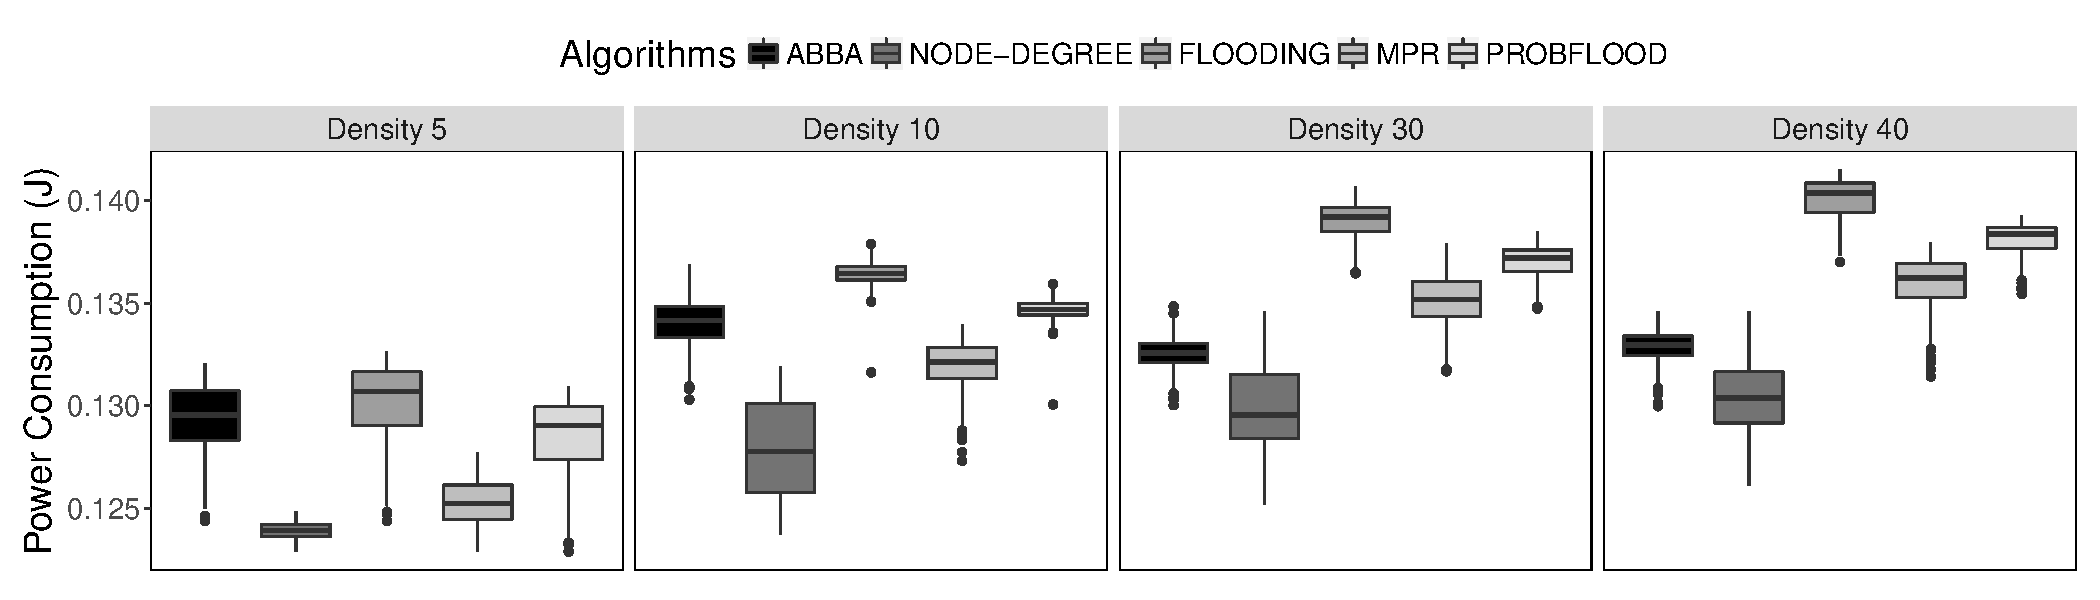
\includegraphics[page=1, scale=0.34, trim = 16mm 0 10mm 0]{fig/results-mobility.pdf}
	}
	\caption{Power consumption and node reachability per algorithm}
	\label{fig:energy-coverage}
	\end{center}
\end{figure*}

%\begin{figure*}[ht]
%	\begin{center}
%		\subfigure[Static Scenarios]{
%			\label{fig:a-sessionTime}
%			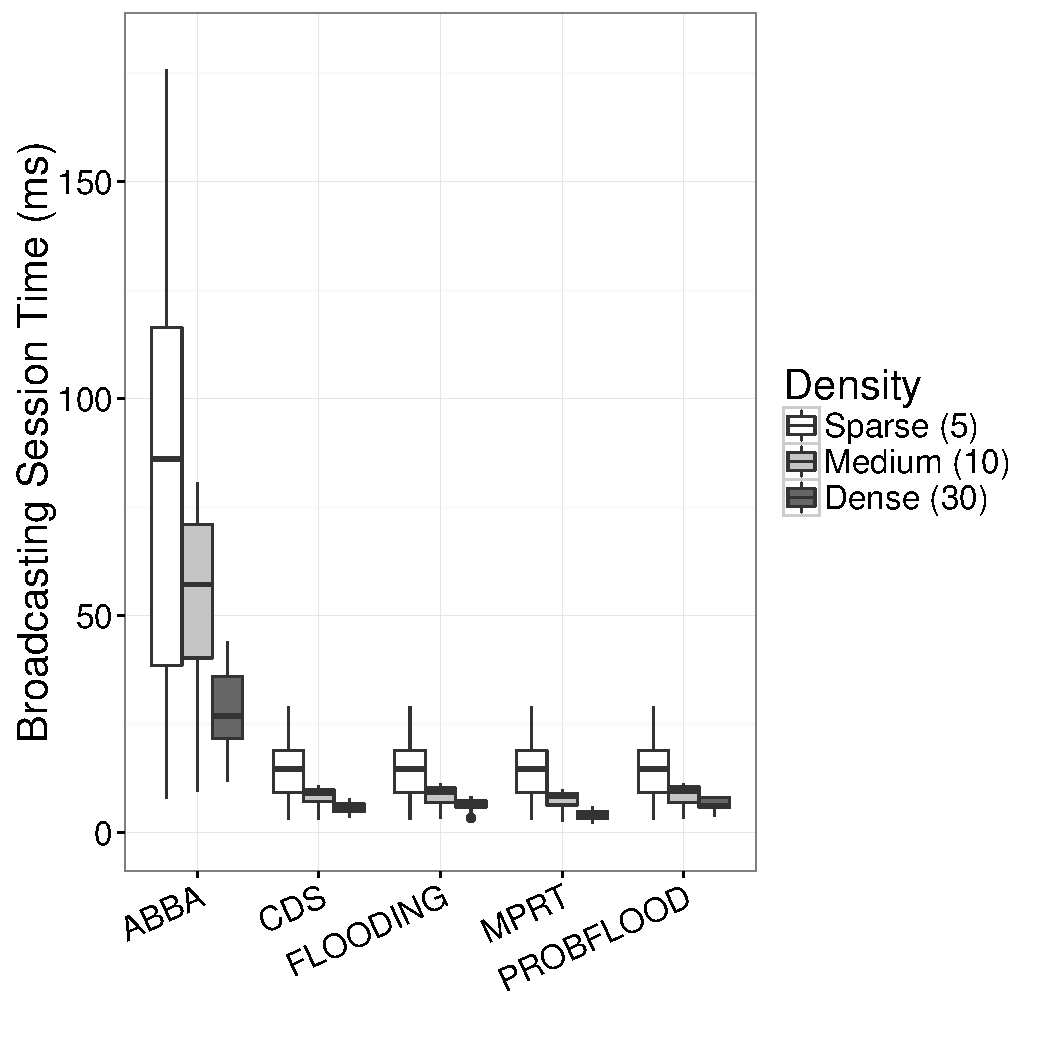
\includegraphics[scale=0.32, trim = 0 0 70mm 0]{fig/SessionTimeNoMob.pdf}
%		}
%		~
%		\subfigure[Dynamic Scenarios]{
%			\label{fig:b-sessionTime}
%			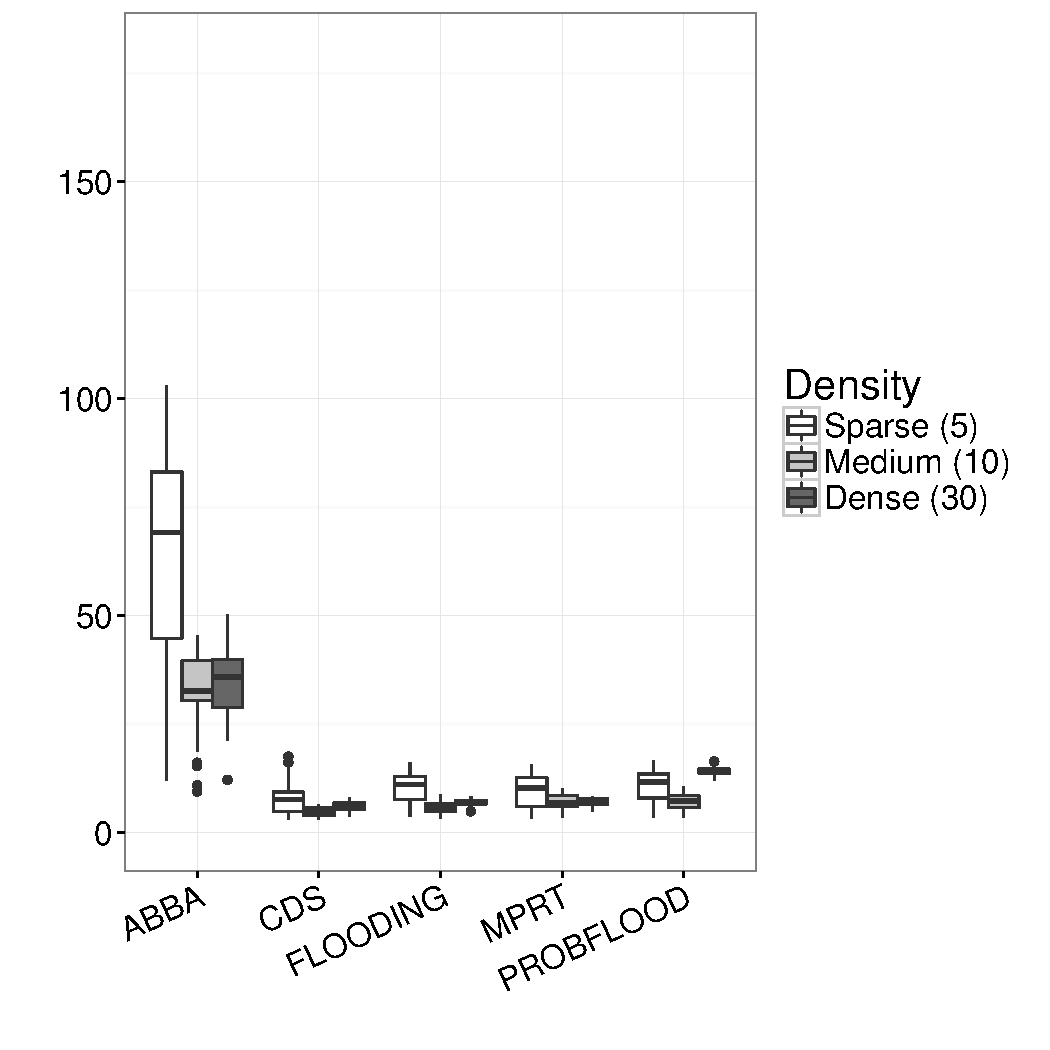
\includegraphics[scale=0.32, trim = 0 0 0 0]{fig/sessionTimeMob.pdf}
%		}
%		\caption{Broadcasting session time}
%		\label{fig:coverage-energy}
%	\end{center}
%\end{figure*}

Figures~\ref{fig:a-energy} and~\ref{fig:b-energy} show the values of energy consumption for the static and mobility settings.
%
We use \textit{violin plots} to present the full distribution of power consumption.
%
Due to space limitations, we only show the results for those densities where there is a significant change in the patterns of energy consumption.
% 
The first thing to note is that, as expected, \textit{simple flooding} consumes more energy in all scenarios.
%
Also interesting is that topology-based approaches, namely \textit{MPR} and \textit{CDS-based}, always outperform other approaches when there is no mobility.
%
This is consistent with the results depicted in Figures~\ref{fig:a-saved} and~\ref{fig:a-duplicated}, which show that nodes send and receive fewer messages in these approaches.
%
In the case of \textit{ABBA} and \textit{ProbFlood}, our experiments do not show a single value of density where these algorithms behave better than \textit{MPR}.
%
This clearly indicates that using control messages to build an underlying topology is worth in terms of power consumption when there is no mobility\deleted{the interval among broadcast messages is close to the interval among control messages}.
%

As depicted in Figure~\ref{fig:b-energy}, the behavior of these protocols changes in dynamic scenarios.
%
In such scenarios, \textit{ABBA} outperforms \textit{MPR} when the density is low or medium (5, 10, 15).
%
Only when the density is greater than 20, MPR becomes competitive again.
%
In correlating these results with Figures~\ref{fig:b-saved} and~\ref{fig:b-duplicated} we notice that nodes send fewer messages with \textit{ABBA} than with \textit{MPR}.
%
We also notice that the number of duplicate messages received using different algorithms in dynamic scenarios is closer than that of the static scenarios.
%
%Although This changes when densities above 30 because the control 
%
We can conclude that, since \textit{MPR} cannot maintain a completely up-to-date underlaying topology due to mobility, it fails in reducing the number of relay nodes and the power consumption is high.

These results are of interest because they support the idea that two parameters of a scenario, namely node mobility and ratio $\textit{broadcast-interval}/\textit{control-message-interval}$, may impact the decision of which algorithm to use to broadcast.
%

\subsection{Reachability}

Figures~\ref{fig:a-coverage} and ~\ref{fig:b-coverage} depict the reachability of the five algorithms studied, in both \textit{static} and \textit{dynamic} scenarios.
%
All these algorithms tend to be reliable in static settings and for densities above 10.
%
Some approaches fail to deliver all broadcast messages in settings with very low density because many sections of the network are only connected by a single link that can be a point of failure. 
%
In particular, \textit{ABBA} and \textit{MPR} are more prone to this kind of situations.
%

%\begin{figure*}[!ht]
%	\begin{center}
%		\subfigure[Static scenario.]{
%			\label{fig:a-coverage}
%			
\includegraphics[page=2, scale=0.40, trim = 20mm 11mm 0 0]{fig/results-static-summary.pdf}
%		}
%		~
%		\subfigure[Dynamic scenario.]{
%			\label{fig:b-coverage}
%			\includegraphics[page=2, scale=0.40, trim = 20mm 11mm 0 0]{fig/results-mobility-summary.pdf}
%		}
%		\caption{Node reachability}
%		\label{fig:coverage}
%	\end{center}
%\end{figure*}

The results in the mobility scenarios are less stable.
%
As expected, some protocols such as \textit{MPR} and \textit{CDS-based} behave worse because the underlying topology they build must be constantly updated due to the movement of nodes.
%
We observe this problem for all the densities, but it is clearer for sparser topologies.
%
We can also see that \textit{ABBA} tends to fail with different values of density, although far less than topology-based approaches.
%
\deleted{This is understandable because \textit{ABBA} is an area-based approach where each node uses the location of its neighbors to drive the broadcast process.}
%
Indeed, since the location of each node changes continuously, ABBA occasionally fails in computing the covered area; as a consequence, some messages are not delivered.
This is consistent with previous studies~\cite{YiGerla2003, Garbinato2010}. 




